\documentclass[12pt,aspectratio=169,notheorems]{beamer}
\graphicspath{
	{img}
}

\usetheme[progressbar=frametitle, numbering=fraction]{metropolis}
\usepackage{appendixnumberbeamer}
\usepackage[font=small,labelfont=bf]{caption}
\usepackage{hyperref}

\setbeamercolor{background canvas}{bg=white}

\usepackage{booktabs}
\usepackage[scale=2]{ccicons}

% Change Color of the theme
\usepackage{xcolor}
\definecolor{DarkGrey}{HTML}{353535}
\definecolor{ECNURed}{RGB}{164,31,53}
\definecolor{ECNUBrown}{RGB}{134,117,77}
\setbeamercolor{normal text}{ fg= DarkGrey  }
\setbeamercolor{alerted text}{ fg= ECNURed  }
\setbeamercolor{example text}{ fg= ECNUBrown  }



\title{\LARGE AI Project Report}
\subtitle{Network Intrusion Detection System}
\author{\\ Andrea Mugnai \\ Jacopo Tucci}
\date{2024/2025}
\titlegraphic{\hfill
\includegraphics[height=2cm]{logo.png}}

\begin{document}

\maketitle

\begin{frame}{Goals}
    Our goal is to create a Network Intrusion Detection System (NIDS) capable of classifying raw network packets into the following categories:
    \begin{itemize}
        \item Normal
        \item Denial of Service (DoS)
        \item User to Root (U2R)
        \item Remote to Local (R2L)
        \item Probe
    \end{itemize}
    The classification models used for this task are based on \textbf{supervised learning}.
\end{frame}

\begin{frame}{Dataset}
    We used a non cleaned dataset: \href{https://research.unsw.edu.au/projects/unsw-nb15-dataset}{UNSW-NB15}. 
    The raw packet was created by the \texttt{IXIA PerfectStorm tool}. This dataset is a labeled datset and in particular has nine types of attacks 
    that we mapped in the categories we mentioned before as follows:
    \begin{itemize}
        \item DoS: DoS, Worms.
        \item U2R: Backdoor, Shellcode.
        \item R2L: Exploits, Analysis.
        \item Probe: Reconnaissance, Fuzzers, Generic.
    \end{itemize}
        We identified 49 features in the dataset, 42 of which are numerical and 7 are categorical.
\end{frame}

\begin{frame}{Category Distribution}
    \begin{center}
        \footnotesize The dataset is highly unbalanced, with the majority of the samples belonging to the \textbf{Normal}.
        
        \hspace*{-0.8cm}
        \begin{minipage}[t][6cm][t]{0.5\textwidth}
            \centering
            \vspace{-0.08cm}
            \fbox{ % Adds a border around the table
                \resizebox{1.2\textwidth}{!}{%
                    \begin{tabular}{|l|l|l|l|l|l|l|l|l|l|}
                        \hline
                        \textbf{Normal} & \textbf{Generic} & \textbf{Exploits} & \textbf{Fuzzers} & \textbf{Reconnaissance} & \textbf{DoS} & \textbf{Backdoor} & \textbf{Analysis} & \textbf{Shellcode} & \textbf{Worms} \\
                        \hline
                        281,462 & 6,894 & 6,851 & 4,970 & 3,420 & 1,465 & 623 & 621 & 371 & 42 \\
                        \hline
                    \end{tabular}
                }
            }
            \caption{Counts for each attack category.}
            \label{tab:inverted_attack_categories}

            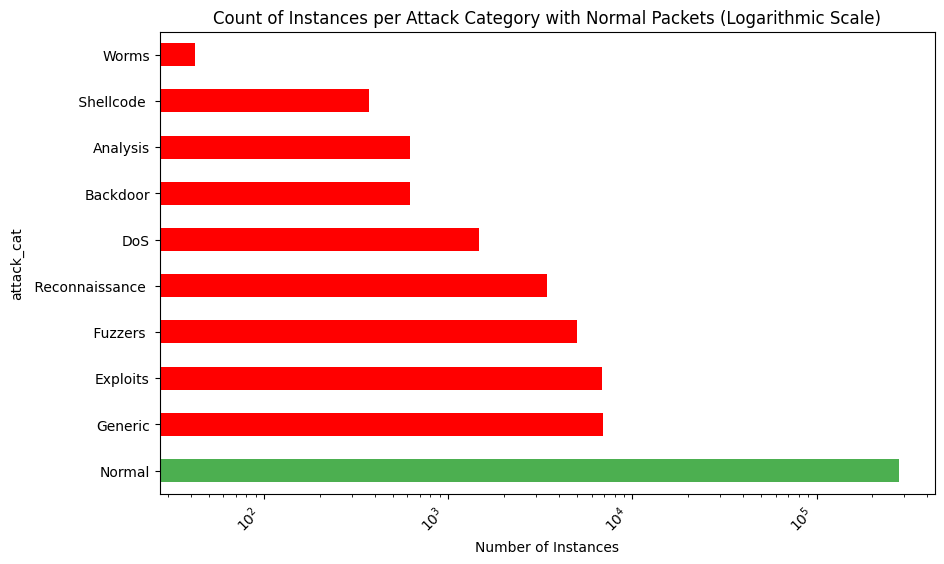
\includegraphics[width=\textwidth, height=5cm, keepaspectratio]{attack_cat_before.png} \\
            \textit{Original Dataset \emph{attack category} distribution}
        \end{minipage} 
        \hfill
        \begin{minipage}[t]{0.45\textwidth}
            \centering
            \vspace{-0.01cm}
            \fbox{ % Adds a border around the table
                \resizebox{0.7\textwidth}{!}{%
                    \begin{tabular}{|l|l|l|l|l|l|}
                        \hline
                        \textbf{Normal} & \textbf{Probe} & \textbf{R2L} & \textbf{DoS} & \textbf{U2R} \\
                        \hline
                        281,462 & 15,284 & 7,472 & 1,507 & 994 \\
                        \hline
                    \end{tabular}
                }
            }
            \caption{Counts for each attack category.}
            \label{tab:inverted_attack_categories}
            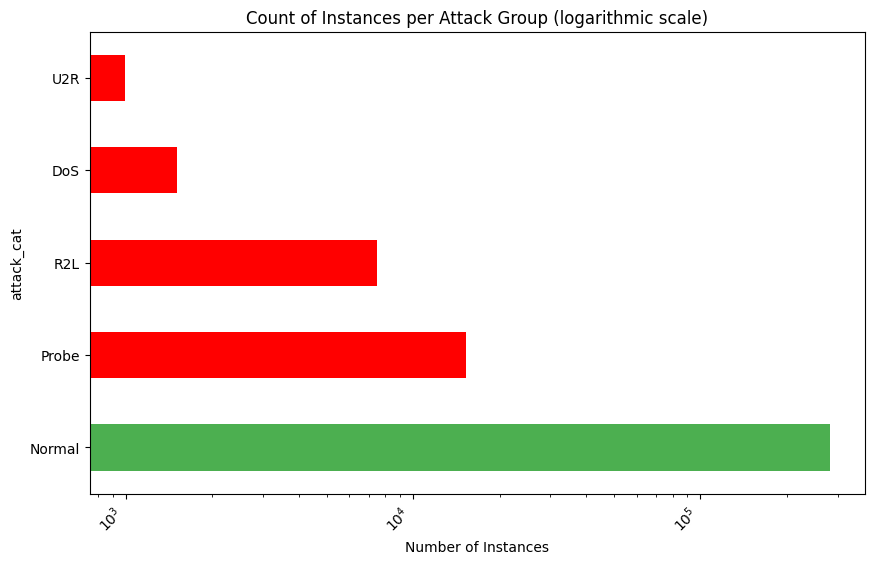
\includegraphics[width=\textwidth, height=4.5cm, keepaspectratio]{attack_cat_after.png} \\
            \textit{Our Dataset \emph{attack category} distribution}
            
        \end{minipage}
        \hspace*{-1cm}
        
    \end{center}
\end{frame}



\begin{frame}{Architecture}
    \begin{center}
        \includegraphics[scale=.65]{architecture-v1.png}
    \end{center}
\end{frame}

\begin{frame}{Architecture - details}
    The \textbf{authentication} component allows to log-in and log-out players and admins. \\[1ex]
    Using \textbf{account}, a player can check his own gacha collection and the transactions history. In particular, a transaction record is created only when an auction is completed (gacha rolls and currency purchasing are not considered as transactions). \\[1ex]
    The \textbf{market} component allows to discover active auctions and make bids, whereas \textbf{currency} component is used to purchase in-game currency. \\[1ex]
    The system gacha collection can be explored through \textbf{collection} component, which allows also to roll new gachas.
\end{frame}

\begin{frame}{Database}
    The gacha app is based on a single relational database which contains all the data inside different tables. In particular, we defined 6 main tables, i.e. \textbf{Player}, \textbf{Gacha}, \textbf{Auction}, \textbf{Transaction}, \textbf{Rarity} and \textbf{Admin}. Related to them, there are 2 \emph{join tables}, i.e. \textbf{Player\_Gacha} and \textbf{Player\_Auction}, which allow to maintain the user's gacha collection and user's bids. \\[1ex]
    An admin can only manage the application and \textbf{cannot} collect/buy gachas. \\[1ex]
    In the next slide we introduce the ER diagram and a brief description of it.  
\end{frame}

\begin{frame}{Database - ER diagram}
    \begin{center}
        \includegraphics[scale=.5]{ASE-er-v4.png}
    \end{center}
\end{frame}

\begin{frame}{Database - ER diagram details}
    The \emph{N-to-N} relationship between \textbf{Player} and \textbf{Gacha} will be implemented with the table \textbf{Player\_Gacha}. The \textbf{Player\_Auction} table expresses the \emph{N-to-N} relationship between \textbf{Player} and \textbf{Auction}. When a player wins an auction and pays the gacha, a transaction record will be created. \\[1ex]
    Each auction is created by one player (i.e. \emph{create} relationship) and it will contain a reference to a transaction record when the winning player pays the bid. For \textbf{Transaction} records, we store the creation datetime. \\[1ex]
    The gacha's rarities are stored inside \textbf{Rarity} table and each gacha maintains a reference to a specific rarity.
\end{frame}

\begin{frame}{User's interactions}
      A player can do a bid only if he has enough currency. The payment operation will be done automatically by the system at the end of the auction. If he cannot pay (e.g. due to no found), the runner-up player will become the winner. \\[1ex]
     We consider in-coming transactions (i.e. player sells a gacha) and out-going ones (i.e. player buys a gacha). In the OpenAPI specifications, we use \textbf{from} and \textbf{to} attributes to distinguish between them.
\end{frame}

\end{document}
